\documentclass[10pt,usenames,dvipsnames]{beamer}

\usetheme[progressbar=frametitle]{metropolis}

\definecolor{ubcBlue}{RGB}{12,35,68}
\definecolor{ubcBlue1}{RGB}{0,85,183}
\definecolor{ubcBlue2}{RGB}{0,167,225}
\definecolor{ubcBlue3}{RGB}{64,180,229}
\definecolor{ubcBlue4}{RGB}{110,196,232}
\definecolor{ubcBlue5}{RGB}{151,212,223}

% \setbeamercolor{normal text}{bg=ubcBlue1}
\setbeamercolor{alerted text}{bg=ubcBlue1, fg = ubcBlue}
\setbeamercolor{example text}{fg=ubcBlue1, bg=ubcBlue1}
\setbeamercolor{title separator}{fg = ubcBlue, bg=ubcBlue}
\setbeamercolor{progress bar}{bg=ubcBlue4, fg=ubcBlue1}
\setbeamercolor{progress bar in head/foot}{bg=ubcBlue4, fg=ubcBlue1}
\setbeamercolor{progress bar in section page}{bg=ubcBlue4, fg=ubcBlue1}
\setbeamercolor{frametitle}{bg=ubcBlue}


\usepackage{appendixnumberbeamer}

\usepackage{booktabs}
\usepackage[scale=2]{ccicons}

\usepackage{pgfplots}
\usepgfplotslibrary{dateplot}

\usepackage{xspace}
\newcommand{\themename}{\textbf{\textsc{metropolis}}\xspace}

%% My Packages
% Text
\usepackage{titlecaps}
% Mathematics and Symbols
\usepackage{amssymb}
\usepackage{amsmath}
\usepackage{amsthm}
\usepackage{mathtools}
\usepackage[electronic]{ifsym}
\usepackage{algorithm}
\usepackage{algpseudocode}
% Time and Units
\usepackage{datetime2}
\usepackage{siunitx}
\sisetup{detect-all}
% Tables
%\usepackage{tabularx}
\newcolumntype{P}[1]{>{\RaggedRight\arraybackslash}p{#1}} % ragged-right version of "p" column type
\newcolumntype{C}[1]{>{\centering\arraybackslash$}p{#1}<{$}} % For fixed-width array columns.
\usepackage{multicol}
\usepackage{multirow}
\usepackage{diagbox}
\usepackage{threeparttable}
\usepackage{makecell}
% Page Formatting
\usepackage{rotating}
\usepackage{pdflscape}
\usepackage{subcaption}
\usepackage{fancyhdr}
\usepackage{ragged2e}
\usepackage{varwidth}
% Graphics and Drawing
\graphicspath{ {img/} }	
\usepackage{tikz}
\usetikzlibrary{arrows, positioning, dsp, chains, fit, calc, matrix}
\usepackage[american]{circuitikz}
\usepackage{pgfplots}
\pgfplotsset{compat=1.3}
\usepgfplotslibrary{fillbetween}
\pgfdeclarelayer{bg}    % declare background layer
\pgfsetlayers{bg,main}  % set the order of the layers (main is the standard layer)
\usepackage{epstopdf}
\epstopdfsetup{outdir=./}
% Files
\usepackage{filecontents}

%% My Macros
% Allow augmented matrix notation
\makeatletter
\renewcommand*\env@matrix[1][*\c@MaxMatrixCols c]{%
  \hskip -\arraycolsep
  \let\@ifnextchar\new@ifnextchar
  \array{#1}}
\makeatother

\makeatletter
\newsavebox{\mybox}
\setbeamertemplate{frametitle}{%
  \nointerlineskip%
  \savebox{\mybox}{%
      \begin{beamercolorbox}[%
          wd=\paperwidth,%
          sep=0pt,%
          leftskip=\metropolis@frametitle@padding,%
          rightskip=\metropolis@frametitle@padding,%
        ]{frametitle}%
      \metropolis@frametitlestrut@start\insertframetitle\metropolis@frametitlestrut@end%
      \end{beamercolorbox}%
    }
  \begin{beamercolorbox}[%
      wd=\paperwidth,%
      sep=0pt,%
      leftskip=\metropolis@frametitle@padding,%
      rightskip=\metropolis@frametitle@padding,%
    ]{frametitle}%
  \metropolis@frametitlestrut@start\insertframetitle\metropolis@frametitlestrut@end%
  \hfill%
  \raisebox{-\metropolis@frametitle@padding}{\includegraphics[height=\dimexpr\ht\mybox+\metropolis@frametitle@padding\relax]{UBC-Metropolis-Beamer/2_2016_UBCNarrow_Signature_ReverseCMYK}}%
    \hspace*{-\metropolis@frametitle@padding}
  \end{beamercolorbox}%
}
\makeatother

\newcommand{\mytitle}{On the Design of Stable, High Performance Sigma Delta Modulators}
\newcommand{\myname}{Brett Hannigan}

\setbeamertemplate{frame footer}{\mytitle\ --- \myname}

\title{\mytitle}
\subtitle{M.A.Sc. Thesis Defence}
\date{\DTMdisplaydate{2018}{12}{04}{}}
\author{\myname\\ \texttt{bch@alumni.ubc.ca}}
\institute{School of Biomedical Engineering\\ University of British Columbia}
% \titlegraphic{\hfill\includegraphics[height=1.5cm]{logo.pdf}}

\begin{document}

\maketitle

\begin{frame}{Table of Contents}
	\setbeamertemplate{section in toc}[sections numbered]
	%\tableofcontents[hideallsubsections]
	\tableofcontents
\end{frame}

\section{Introduction}

\begin{frame}[fragile]{Project Objectives}

\metroset{block=fill}
\begin{center}
	
\includegraphics[width=6cm]{logos.png}
\end{center}
\begin{block}{Primary Objective}
	To develop a systematic method of design for sigma delta A/D converters for the recording of bio-signals.
\end{block}
Ideally, the goals of the method are to:
\begin{itemize}
	\item Model the nonlinear system accurately in a way that allows analysis of existing designs.
	\item Reduce dependence on simulation.
	\item Provide a way to design guaranteed stable sigma delta modulators in a way that minimizes conservatism.
\end{itemize}

\end{frame}

\begin{frame}{Principles of Sigma Delta Modulation}

\begin{figure}
\noindent\makebox[\textwidth]{
	\centering
	\begin{tikzpicture}[ampersand replacement=\&,scale=0.75, every node/.style={scale=0.75}]
		\node[coordinate] (g-y0) at (0,0) {};
		\node[coordinate] (g-y1) at (5,0) {};
		\node[coordinate] (g-y2) at (10,0) {};
		\begin{axis}[
			at={(g-y0)},
			anchor=center,
			width=6cm, height=3.75cm,
			anchor=center, 
			xmin=0, xmax=4,
			ymin=-100, ymax=300,
			axis x line=none, axis y line=none, axis line style={-},
			xticklabels={0,1,2,3,\SI{4}{\second}}, xtick={0,1,2,3,4},
			yticklabels={, 0, \SI{300}{\micro\volt}}, ytick={-100, 0, 300}
			]
			\addplot[solid,black] table [x=t, y=y, col sep=comma] {data/comparison-y0.csv};
		\end{axis}
		
		\begin{axis}[
			at={(g-y1)},
			anchor=center,
			width=6cm, height=3.75cm,
			anchor=center, 
			xmin=0, xmax=4,
			ymin=-100, ymax=300,
			axis x line=none, axis y line=none, axis line style={-},
			xticklabels={0,1,2,3,\SI{4}{\second}}, xtick={0,1,2,3,4},
			yticklabels={, 0, \SI{300}{\micro\volt}}, ytick={-100, 0, 300}
			]
			\addplot[solid,black] table [x=t, y=y, col sep=comma] {data/comparison-y1.csv};
		\end{axis}
		
		\begin{axis}[
			at={(g-y2)},
			anchor=center,
			width=6cm, height=3.75cm,
			anchor=center, 
			xmin=0, xmax=4,
			ymin=-100, ymax=300,
			axis x line=none, axis y line=none, axis line style={-},
			xticklabels={0,1,2,3,\SI{4}{\second}}, xtick={0,1,2,3,4},
			yticklabels={, 0, \SI{300}{\micro\volt}}, ytick={-100, 0, 300}
			]
			\addplot[solid,black] table [x=t, y=y, col sep=comma] {data/comparison-y2.csv};
		\end{axis}
		
	\end{tikzpicture}}
	\caption{An example EEG signal \cite{Blankertz2007} digitized to 5 bits with na\"{i}ve quantization (left), 10 times oversampled quantization (middle), and first-order sigma delta modulation (right).}
\end{figure}
\metroset{block=fill}
\begin{block}{Oversampling}
	Sampling a signal at a rate higher than what the Nyquist-Shannon sampling theorem would dictate.
\end{block}
\begin{block}{Noise Shaping}
	The use of a filter to push quantization noise out of the signal band by wrapping the quantizer in a feedback loop.
\end{block}

\end{frame}

\begin{frame}{Basic Structure of a Sigma Delta Modulator}

\begin{figure}
\noindent\makebox[\textwidth]{
	\centering
	\begin{tikzpicture}[ampersand replacement=\&,scale=0.75, every node/.style={scale=0.75}]
		\matrix (m2) at (0,0) [row sep=0mm, column sep=5mm, matrix anchor=north west]
		{
			%-----------------------------------------------------------------------------------------------------------------------------------------------
			\node[coordinate]								(m2-00) {};							\&
			\node[coordinate]								(m2-01) {};							\&
			\node[coordinate,label={above:\PulseHigh \ $OSR \cdot f_s$}]	(m2-02) {};							\&
			\node[coordinate]								(m2-03) {};							\&
			\node[coordinate]								(m2-04) {};							\&
			\node[dspnodeopen]							(m2-05) {};							\& \\
			%------------------------------------------------------------------------------------------------------------------------------------------------
			\node[dspnodeopen,color=Red]						(m2-10) {};							\&
			\node[dspsquare,label={above:AAF}]					(m2-11) {};							\&
			\node[dspsquare]								(m2-12) {S/H};						\&
			\node[dspadder,label={below left:$-$}]				(m2-13) {};							\&
			\node[dspsquare,label={above:LF}]					(m2-14) {$\int$};						\&
			\node[dspsquare]								(m2-15) {\RaisingEdge};					\&
			\node[dspnodefull,color=ForestGreen]					(m2-16) {};							\&
			\node[dspsquare,label={above:DRF}]					(m2-17) {};							\&
			\node[dspfilter]								(m2-18) {$\downarrow OSR$};				\&
			\node[dspnodeopen,color=Blue]						(m2-19) {};							\& \\
			%------------------------------------------------------------------------------------------------------------------------------------------------
			\node[coordinate]								(m2-20) {};							\&
			\node[coordinate]								(m2-21) {};							\&
			\node[coordinate]								(m2-22) {};							\&
			\node[coordinate]								(m2-23) {};							\&
			\node[coordinate]								(m2-24) {};							\&
			\node[coordinate]								(m2-25) {};							\&
			\node[coordinate]								(m2-26) {};							\& \\
			%------------------------------------------------------------------------------------------------------------------------------------------------
		};
		
		\draw[->] (m2-02) -- (m2-12);
		\draw[dspconn] (m2-05) -- (m2-15);
		\draw[dspconn,color=Red] (m2-10) -- (m2-11);
		\draw[dspconn,color=Red] (m2-11) -- (m2-12);
		\draw[dspconn,color=ForestGreen] (m2-12) -- (m2-13);
		\draw[dspconn,color=ForestGreen] (m2-13) -- (m2-14);
		\draw[dspconn,color=ForestGreen] (m2-14) -- (m2-15);
		\draw[dspline,color=ForestGreen] (m2-15) -- (m2-16);
		\draw[dspconn,color=ForestGreen] (m2-16) -- (m2-17); 
		\draw[dspconn,color=ForestGreen] (m2-17) -- (m2-18);
		\draw[dspconn,color=Blue] (m2-18) -- (m2-19);
		\draw[dspline,color=ForestGreen] (m2-16) -- (m2-26);
		\draw[dspline,color=ForestGreen] (m2-26) -- (m2-23);
		\draw[dspconn,color=ForestGreen] (m2-23) -- (m2-13);
		
		\node[draw,inner xsep=15pt,inner ysep=10pt,dashed,fit={($(m2-05.north)+(-0.3,0)$) ($(m2-15.south)+(0.3,0.1)$)},label={[align=center]above:Linear Model}] {};
		
		\pgfplotsset{width=2.25cm,height=2.25cm,xmin=0.1,xmax=1000000,ymin=0.0001,ymax=10}
		\begin{loglogaxis}[
				at={($(m2-11) + (-9,-9)$)},
				ticks=none,
				axis x line*=bottom,
				axis y line*=left
			 ]
			\addplot[domain=1:100000]  {(60*x+10000)/(x*x + 60*x+10000)};
		\end{loglogaxis}
		\pgfplotsset{width=2.25cm,height=2.25cm,xmin=0.1,xmax=1000000,ymin=0.0001,ymax=10}
		\begin{loglogaxis}[
				at={($(m2-17) + (-9,-9)$)},
				ticks=none,
				axis x line*=bottom,
				axis y line*=left
			 ]
			\addplot[domain=1:100000]  {(60*x+10000)/(x*x + 60*x+10000)};
		\end{loglogaxis}

		\draw[Gray, ->, out=0, in=90, looseness=0.85] ($(m2-05)+(0.25, 0)$) to node[above,xshift=5pt] {NTF} ($(m2-16)+(0.4, 0.25)$);
		\draw[Gray, ->, out=-45, in=-90, looseness=0.5] ($(m2-12)+(1,-0.25)$) to node[below] {STF} ($(m2-16)+(0.4,-0.25)$);

	\end{tikzpicture}}
	\caption{A simplified block diagram of a discrete-time sigma delta A/D converter.}
\end{figure}
\vspace{-0.75cm}
\begin{figure}
\noindent\makebox[\textwidth]{
	\centering
	\begin{tikzpicture}[ampersand replacement=\&,scale=0.75, every node/.style={scale=0.75}]
		\matrix (m2) at (0,0) [row sep=0mm, column sep=5mm, matrix anchor=north west]
		{
			%-----------------------------------------------------------------------------------------------------------------------------------------------
			\node[coordinate]								(m2-00) {};							\&
			\node[coordinate]								(m2-01) {};							\&
			\node[coordinate]								(m2-02) {};							\&
			\node[coordinate]								(m2-03) {};							\&
			\node[coordinate,label={above:\PulseHigh \ $OSR \cdot f_s$}]	(m2-04) {};							\&
			\node[dspnodeopen]							(m2-05) {};							\& \\
			%------------------------------------------------------------------------------------------------------------------------------------------------
			\node[dspnodeopen,color=Red]						(m2-10) {};							\&
			\node[dspsquare,dashed,label={above:AAF}]				(m2-11) {};							\&
			\node[dspadder,label={below left:$-$}]				(m2-12) {};							\&
			\node[dspsquare,label={above:LF}]					(m2-13) {$\int$};						\&
			\node[dspsquare]								(m2-14) {S/H};						\&
			\node[dspsquare]								(m2-15) {\RaisingEdge};					\&
			\node[dspnodefull,color=ForestGreen]					(m2-16) {};							\&
			\node[dspsquare,label={above:DRF}]					(m2-17) {};							\&
			\node[dspfilter]								(m2-18) {$\downarrow OSR$};				\&
			\node[dspnodeopen,color=Blue]						(m2-19) {};							\& \\
			%------------------------------------------------------------------------------------------------------------------------------------------------
			\node[coordinate]								(m2-20) {};							\&
			\node[coordinate]								(m2-21) {};							\&
			\node[coordinate]								(m2-22) {};							\&
			\node[coordinate]								(m2-23) {};							\&
			\node[dspadc]								(m2-24) {D/A};							\&
			\node[coordinate]								(m2-25) {};							\&
			\node[coordinate]								(m2-26) {};							\& \\
			%------------------------------------------------------------------------------------------------------------------------------------------------
		};
		
		\draw[->] (m2-04) -- (m2-14);
		\draw[dspconn] (m2-05) -- (m2-15);
		\draw[dspconn,color=Red] (m2-10) -- (m2-11);
		\draw[dspconn,color=Red] (m2-11) -- (m2-12);
		\draw[dspconn,color=Red] (m2-12) -- (m2-13);
		\draw[dspconn,color=Red] (m2-13) -- (m2-14);
		\draw[dspconn,color=ForestGreen] (m2-14) -- (m2-15);
		\draw[dspline,color=ForestGreen] (m2-15) -- (m2-16);
		\draw[dspconn,color=ForestGreen] (m2-16) -- (m2-17); 
		\draw[dspconn,color=ForestGreen] (m2-17) -- (m2-18);
		\draw[dspconn,color=Blue] (m2-18) -- (m2-19);
		\draw[dspline,color=ForestGreen] (m2-16) -- (m2-26);
		\draw[dspconn,color=ForestGreen] (m2-26) -- (m2-24);
		\draw[dspline,color=Red] (m2-24) -- (m2-22);
		\draw[dspconn,color=Red] (m2-22) -- (m2-12);
		\pgfplotsset{width=2.25cm,height=2.25cm,xmin=0.1,xmax=1000000,ymin=0.0001,ymax=10}
		
		\node[draw,inner xsep=15pt,inner ysep=10pt,dashed,fit={($(m2-05.north)+(-0.3,0)$) ($(m2-15.south)+(0.3,0.1)$)},label={[align=center]above:Linear Model}] {};
		
		\begin{loglogaxis}[
				at={($(m2-11) + (-9,-9)$)},
				ticks=none,
				axis x line*=bottom,
				axis y line*=left
			 ]
			\addplot[domain=1:100000]  {(60*x+10000)/(x*x + 60*x+10000)};
		\end{loglogaxis}
		\pgfplotsset{width=2.25cm,height=2.25cm,xmin=0.1,xmax=1000000,ymin=0.0001,ymax=10}
		\begin{loglogaxis}[
				at={($(m2-17) + (-9,-9)$)},
				ticks=none,
				axis x line*=bottom,
				axis y line*=left
			 ]
			\addplot[domain=1:100000]  {(60*x+10000)/(x*x + 60*x+10000)};
		\end{loglogaxis}

		\draw[Gray, ->, out=0, in=90, looseness=0.85] ($(m2-05)+(0.25, 0)$) to node[above,xshift=5pt] {NTF} ($(m2-16)+(0.4, 0.25)$);
		\draw[Gray, ->, out=-75, in=-90, looseness=0.8] ($(m2-11)+(1,-0.25)$) to node[above] {STF} ($(m2-16)+(0.4,-0.25)$);

	\end{tikzpicture}}
	\vspace{-1cm}
	\caption{A simplified block diagram of a continuous-time sigma delta A/D converter.}
\end{figure}

\end{frame}

\begin{frame}{Design of the Loop Filter}
	The nonlinear quantizer in the forward path makes stability analysis difficult.
	Loop filter design is commonly done in one of several ways:
	\begin{itemize}
		\item Pure integrator -- DC-stable for low order loops \cite{Hein1993}.
		\item Prototype NTF -- noise rejection of linear model chosen from a family of filters \cite[Appx. B]{Schreier1997}.
		\item Optimization-based approaches -- wide range of techniques.
	\end{itemize}
	The design process often relies on extensive simulation to confirm that stability is likely during normal operation and the circuit may include complicated instability detection and recovery mechanisms \cite{Wong2004, Sooch1989, Moussavi1994, Eynde1991}.
\end{frame}

\section{Stability and Performance}

\begin{frame}{$\mathcal{H}_\infty$ Stability Criterion}

\metroset{block=fill}
\begin{block}{$\mathcal{H}_\infty$ Stability Criterion}
	\emph{Lee's rule} states that a modulator is probably stable if the peak of the NTF frequency response is less than a heuristic value.
	\begin{equation*}
		||NTF(z)||_\infty \lessapprox 2
	\end{equation*}
\end{block}

\begin{itemize}
	\item Rule-of-thumb developed empirically from observations on a 4th order DT modulator \cite{Chao1990}.
	\item Generally conservative for 2nd order loops, approximately correct for 3rd order, and inadequate for higher order \cite{Schreier1993}.
	\item Common in existing design tools \cite[Appx. B]{Schreier1997}.
	\item Easy to apply as a control optimization problem.
	\item No straightforward relationship between maximum stable input and the Lee criterion value.
\end{itemize}

\end{frame}

\begin{frame}{Root Locus Stability Criterion}

\metroset{block=fill}
\begin{block}{Root Locus Stability Criterion}
	The describing function of the nonlinear quantizer is a variable gain dependent on quantizer input amplitude. A modulator loop is stable if the root locus remains in the stable region of the complex plane when sweeping through valid quantizer gains.
	\begin{equation*}
		|NTF(z, K)| \leq 1 \quad \forall K \in [k_l, k_h]
	\end{equation*}
\end{block}

\begin{itemize}
	\item Has been used to produce designs by examining pole and zero departure angles \cite{Yang2002, Kuo2006, Kang2014}.
	\item Can predict the maximum stable input amplitude.
\end{itemize}

\end{frame}

\begin{frame}{$\mathcal{H}_2$ Stability Criterion}

\metroset{block=fill}
\begin{block}{$\mathcal{H}_2$ Stability Criterion}
	The $\mathcal{H}_2$ stability criterion predicts stability for a class of norm-bounded input signals $r$ if the squared 2-norm (power gain) of the NTF is less than a value calculated by placing assumptions on the statistical distribution of the quantizer input signal $u$.
	\begin{equation*}
		||NTF(z)||_2^2 \leq f(r,u)
	\end{equation*}
\end{block}

\begin{itemize}
	\item Splits signals into DC baseline with superposition of the AC component, uses additional degrees of freedom to enforce that the quantization error is uncorrelated with quantizer input \cite{Risbo1994}.
	\item A good approximation as long as the chosen quantizer input PDF is accurate.
	\item Can predict the maximum stable input amplitude.
\end{itemize}

\end{frame}

\begin{frame}{$\ell_1$ Stability Criterion}

\metroset{block=fill}
\begin{block}{$\ell_1$ Stability Criterion}
	The input to the quantizer can be bounded for a class of norm-bounded input signals $r$ if the absolute value of the sum of loop filter impulse response coefficients (maximum peak-to-peak gain) is bounded .
	\begin{equation*}
		\min_K ||ntf_K[n]||_1 \leq 3 - ||r||_\infty
	\end{equation*}
\end{block}

\begin{itemize}
	\item Sufficient criterion for BIBO stability \cite{Anastassiou1989}.
	\item Uses the worst-case gain of the filter, usually resulting in very conservative designs \cite{Risbo1994}.
	\item Determines the maximum stable input amplitude.
\end{itemize}

\end{frame}

\begin{frame}{Performance}

\metroset{block=fill}
\begin{block}{Performance Goal}
	\begin{equation*}
		\min ||NTF(z)||_\infty \quad z \in [j\omega_l, j\omega_h]
	\end{equation*}
\end{block}

\begin{itemize}
	\item Want to maximize the quantization noise rejection in the signal band.
	\item Two main options:
	\begin{itemize}
		\item Addition of weighting filters to the NTF channel, then use $\mathcal{H}_\infty$ control techniques.
		\item Apply the Generalized KYP lemma which provides a link between a finite-frequency inequality and a set of LMIs.
	\end{itemize}
\end{itemize}

\end{frame}

\section{Similar Work}

\begin{frame}{Similar Work}

\vspace{-0.8cm}
\begin{table}
\begin{threeparttable}
%\noindent\makebox[\textwidth]{
	\caption{A comparison of some recent work on sigma delta modulator design as a control optimization problem.}
	\begin{tabular}{p{0.5cm} p{1.8cm} p{0.6cm} p{1.9cm} p{3.3cm}}
	%\begin{tabularx}{\textwidth}{X P{1.8cm} P{1.9cm} P{0.7cm} P{3.2cm}}
		\toprule
		\textbf{Ref.} & \textbf{Optimized norms} & \textbf{NTF Type} & \textbf{Performance goal} & \textbf{Stability criteria} \\
		\midrule
		\cite{Oberoi2004} & $\mathcal{H}_\infty$, $\mathcal{H}_2$, $\ell_1$ & IIR &  Weighting filters & $\mathcal{H}_\infty$, $\mathcal{H}_2$ \\ 
		\cite{Osqui2007} & $\mathcal{H}_\infty$ & IIR\tnote{1} & GKYP & Not reported \\
		\cite{Nagahara2012} & $\mathcal{H}_\infty$ & FIR & GKYP & $\ell_1$ mentioned, $\mathcal{H}_\infty$ used \\
		\cite{Li2014} & $\mathcal{H}_\infty$ & IIR & GKYP & $\mathcal{H}_\infty$ \\
		\cite{Tariq2016} & $\mathcal{H}_\infty$, $\mathcal{H}_2$, $\ell_1$ & FIR & Weighting filters & $\ell_1$ mentioned, $\mathcal{H}_\infty$ used \\
		This & $\mathcal{H}_2$, $\ell_1$ & IIR & GKYP & $\mathcal{H}_\infty$, root locus, $\mathcal{H}_2$, $\ell_1$ \\
		\bottomrule
	\end{tabular}
	\begin{tablenotes}
		\item[1] Only the zeros of the IIR filter are optimized.
	\end{tablenotes}
%	}
\end{threeparttable}
\end{table}

\end{frame}

\section{Optimization}

\begin{frame}{Modelling}

\begin{figure}
	\centering
	% Augmented Plant
	\begin{tikzpicture}[ampersand replacement=\&,scale=0.75, every node/.style={scale=0.75}]
	
		% Place nodes using a matrix
		\matrix (m1) [row sep=2.5mm, column sep=5mm]
		{
			%-----------------------------------------------------------------------------------------------
			\node[coordinate]					(m00) {};				\&
			\node[coordinate]					(m01) {};				\&
			\node[dspnodeopen,dsp/label=above]		(m02) {$e$};				\&
			\node[coordinate]					(m03) {};				\&
			\node[dspnodeopen,dsp/label=above]		(m04) {$u$};				\&
			\node[dspsquare]					(m05) {$\Delta$};			\&
			\node[coordinate]					(m06) {};				\& \\
			%-----------------------------------------------------------------------------------------------
			\node[dspnodeopen,dsp/label=left]		(m10) {$r$};				\&
			\node[dspadder,label={below left:$-$}]	(m11) {};				\&
			\node[dspnodefull]					(m12) {};				\&
			\node[dspfilter]					(m13) {$H(z)$};			\&
			\node[dspnodefull]					(m14) {};				\&
			\node[dspfilter,yshift=5]				(m15) {$K$};				\&
			\node[dspnodefull]					(m16) {};				\&
			\node[dspnodeopen,dsp/label=right]		(m17) {$y$};				\& \\
			%-----------------------------------------------------------------------------------------------
			\node[coordinate]					(m20) {};				\&
			\node[coordinate]					(m21) {};				\&
			\node[coordinate]					(m22) {};				\& 
			\node[coordinate]					(m23) {};				\& 
			\node[coordinate]					(m24) {};				\&
			\node[coordinate]					(m25) {};				\& 
			\node[coordinate]					(m26) {};				\& \\
			%-----------------------------------------------------------------------------------------------
		};
		
		\node[draw,inner xsep=15pt,inner ysep=10pt,dashed,fit={($(m10) + (0,0.6)$) ($(m16)+(0.85, -1)$)},label={[align=center]below:Augmented System $G(z)$}] {};
	
		\draw[dspconn] (m10) -- (m11);
		\draw[dspconn] (m11) -- (m13);
		\draw[dspconn] (m12) -- (m02);
		\node[coordinate] at ($(m15) + (-20pt,-5pt)$) (m15-sw) {};
		\node[coordinate] at ($(m15) + (20pt,-5pt)$) (m15-se) {};
		\node[coordinate] at ($(m15) + (-20pt,5pt)$) (m15-nw) {};
		\node[coordinate] at ($(m15) + (20pt,5pt)$) (m15-ne) {};
		\node[coordinate] at ($(m15-nw) + (-10pt,0)$) (m15-nw-corner) {};
		\node[coordinate] at ($(m15-ne) + (10pt,0)$) (m15-ne-corner) {};
		\node[coordinate] at (m15-nw-corner |- m05.west) (m05-w-corner) {};
		\node[coordinate] at (m15-ne-corner |- m05.east) (m05-e-corner) {};
		
		\draw[dspconn] (m13) -- (m15-sw);
		\draw[dspconn] (m15-se) -- (m17);
		\draw[dspconn] (m15-nw-corner) -- (m15-nw);
		\draw[dspline] (m15-nw-corner) -- (m05-w-corner);
		\draw[dspline] (m05) -- node[midway,above] {$w$} (m05-w-corner);
		\draw[dspline] (m15-ne-corner) -- (m15-ne);
		\draw[dspline] (m15-ne-corner) -- (m05-e-corner);
		\draw[dspconn] (m05-e-corner) -- node[midway,above] {$z$} (m05);
		\draw[dspline] (m16) -- (m26);
		\draw[dspline] (m26) -- (m21);
		\draw[dspconn] (m21) -- (m11);
		\draw[dspconn] (m14) -- (m04);
		%\draw[black!20, ->, out=-90, in=-90, looseness=0.6] ($(m10)+(-0.35, -0.25)$) to node[below, xshift=-22pt] {$STF$} ($(m17)+(0.35, -0.25)$);
		%\draw[RedOrange, ->, out=90, in=180, looseness=1] ($(m10)+(-0.35, 0.25)$) to node[left, xshift=-2pt,yshift=2pt] {$NTF$} ($(m02)+(-0.35, 0.35)$);
		
	\end{tikzpicture}
	\caption{The augmented system model with channels of interest extracted.}
\end{figure}
\begin{equation*}
	G:
	\begin{bmatrix}
		\dot{x} \\
		z \\
		e \\
		u \\
		y
	\end{bmatrix} =
	\begin{bmatrix}[c|cc]
		A_H - k_{22}B_HC_H & -k_{21}B_H & B_H \\
		\cmidrule(lr){1-3}
		k_{12}C_H & k_{11} & 0 \\
		-k_{22}C_H & -k_{21} & 1 \\
		C_H & 0 & 0 \\
		k_{22}C_H & k_{21} & 0
	\end{bmatrix}
	\begin{bmatrix}
		x \\
		w \\
		r
	\end{bmatrix}
\end{equation*}

\end{frame}

\begin{frame}{Semidefinite Program}

LMIs exist for the GKYP Lemma \cite{Iwasaki2005}, $\mathcal{H}_2$ norm \cite{Masubuchi1998}, and $\star$-norm \cite{Bu2000, Oberoi2005}, an upper bound of the $\ell_1$ norm, but there are some caveats:
\begin{itemize}
	\item LMIs are non-convex for IIR filters because there is a product term of the pole coefficients.
	\item The $\star$-norm LMI has a non-convex scalar term.
\end{itemize}

\end{frame}

\begin{frame}{Convexification}

The authors in \cite{Li2014} showed how to manipulate the GKYP LMI by assuming the augmented system is in CCF so that there is only one occurrence of the non-convex term in a form like:
\begin{equation*}
	\cdots + 
	\begin{bmatrix}
		\textcolor{Red}{aa^T} & a \\
		a^T & 1
	\end{bmatrix} \geq 0
\end{equation*}
With this reduction, attempted the following:
\begin{itemize}
	\item Use of general non-convex solver.
	\item Use of rank-constrained LMI solver.
	\item Applying Shor's relaxation to linearize the problem.
	\item \textcolor{Violet}{Performing an iterative method \cite{Shishkin2017}.}
\end{itemize}

\end{frame}

\section{Examples}

{\setbeamercolor{background canvas}{bg=white}

\begin{frame}{$\mathcal{H}_\infty$ Stability Criterion i}

\begin{figure}
	\begin{NoHyper}
		\begin{center}
			\begin{tikzpicture}
				\pgfplotsset{set layers}
				\begin{axis}[
					width=1.8in,
					title={\textbf{Trade-off with Lee Stability Criterion}},
					scale only axis,
					xmin=1,xmax=2.2,
					ymin=50,ymax=100,
					axis y line*=left,
					xlabel={Lee criterion},
					ylabel={Maximum SQNR (dB) \ref{plt:msqnr1}},
					]
					\addplot[solid,mark=*,mark options={fill=white}] table [x=lee,y=maxSqnr,col sep=comma] {data/comparison-hinf.csv};
					\label{plt:msqnr1}
					\addplot[mark=*,mark options={fill=black}] coordinates {(1.5, 86)};
				\end{axis}
				\begin{axis}[
					width=1.8in,
					scale only axis,
					xmin=1,xmax=2.2,
					ymin=-50,ymax=0,
					axis y line*=right,
					axis x line=none,
					ylabel={MSIA, relative to FS (dB) \ref{plt:msia1}},
					]
					\addplot[solid,draw=gray,mark=square*,mark options={fill=white}] table [x=lee,y=msia,col sep=comma] {data/comparison-hinf.csv};
					\label{plt:msia1}
					\addplot[mark=square*,draw=gray,mark options={fill=gray}] coordinates {(1.5, -2.975)};
					\end{axis}
			\end{tikzpicture}
		\end{center}
	\end{NoHyper}
	\caption{The performance (maximum simulated SQNR) and stability (simulated MSIA) achieved with the $\mathcal{H}_\infty$ modulator design for different Lee criterion goals.}
\end{figure}

\end{frame}

\begin{frame}{$\mathcal{H}_\infty$ Stability Criterion ii}

\begin{figure}
	\centering
	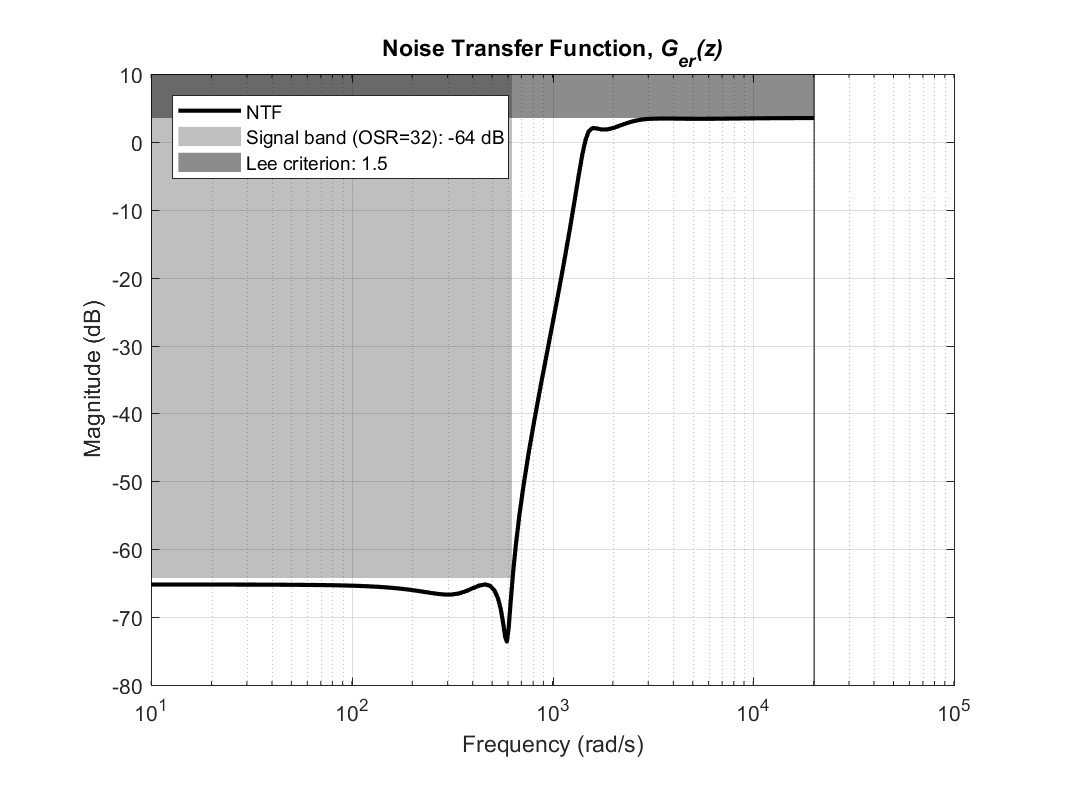
\includegraphics[height=6cm]{ntf-hinf}
	\caption{The noise transfer function generated with the $\mathcal{H}_\infty$ stability criterion and associated optimization targets.}
\end{figure}

\end{frame}

\begin{frame}{$\mathcal{H}_\infty$ Stability Criterion iii}

\begin{figure}
	\centering
	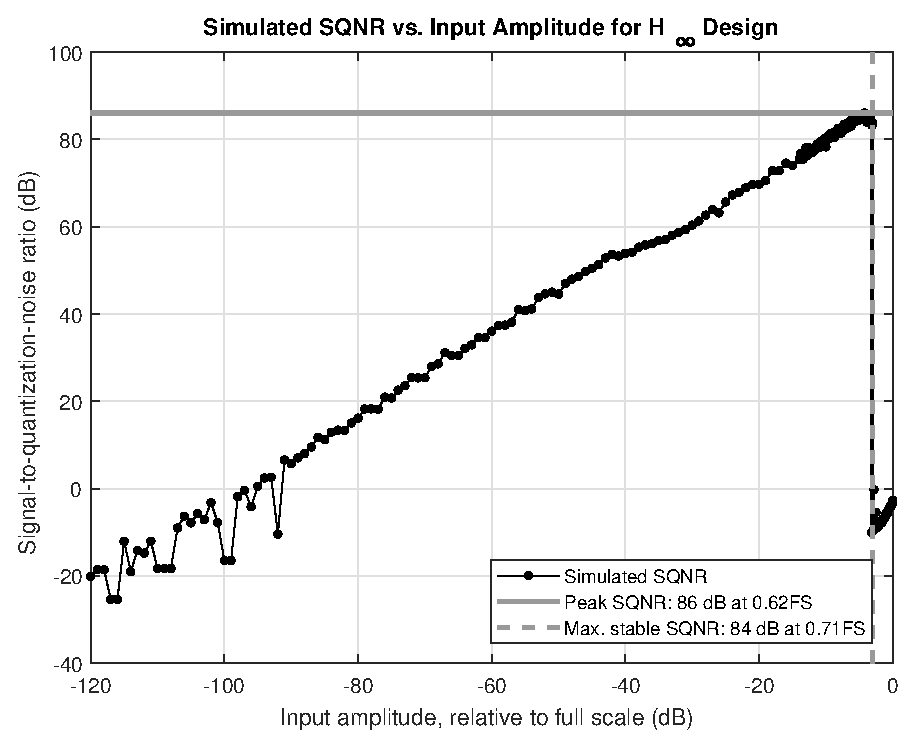
\includegraphics[height=6cm]{sqnr-hinf}
	\caption{Simulation data for the modulator generated with the $\mathcal{H}_\infty$ stability critierion.}
\end{figure}

\end{frame}
}

{\setbeamercolor{background canvas}{bg=white}
\begin{frame}{Root Locus Stability Criterion i}

\begin{figure}
	\begin{NoHyper}
		\begin{center}
			\begin{tikzpicture}
				\pgfplotsset{set layers}
				\begin{axis}[
					width=1.8in,
					title={\textbf{Trade-off with Root Locus Stability Criterion}},
					scale only axis,
					xmin=0,xmax=0.7,
					ymin=40,ymax=100,
					axis y line*=left,
					xlabel={Quantizer gain lower bound $k_l$},
					ylabel={Maximum SQNR (dB) \ref{plt:msqnr2}},
					]
					\addplot[solid,mark=*,mark options={fill=white}] table [x=kl,y=maxSqnr,col sep=comma] {data/comparison-robust.csv};
					\label{plt:msqnr2}
					\addplot[mark=*,mark options={fill=black}] coordinates {(0.1, 65.57)};
				\end{axis}
				\begin{axis}[
					width=1.8in,
					scale only axis,
					xmin=0,xmax=0.7,
					ymin=-80,ymax=0,
					axis y line*=right,
					axis x line=none,
					ylabel={MSIA, relative to FS (dB) \ref{plt:msia2}},
					]
					\addplot[solid,draw=gray,mark=square*,mark options={fill=white}] table [x=kl,y=msia,col sep=comma] {data/comparison-robust.csv};
					\label{plt:msia2}
					\addplot[mark=square*,draw=gray,mark options={fill=gray}] coordinates {(0.1, 0)};
					\end{axis}
			\end{tikzpicture}
		\end{center}
	\end{NoHyper}
	\caption{The performance (maximum simulated SQNR) and stability (simulated MSIA) achieved with the root locus modulator design for different quantizer gain robustness goals.}
\end{figure}

\end{frame}

\begin{frame}{Root Locus Stability Criterion ii}

\begin{figure}
	\centering
	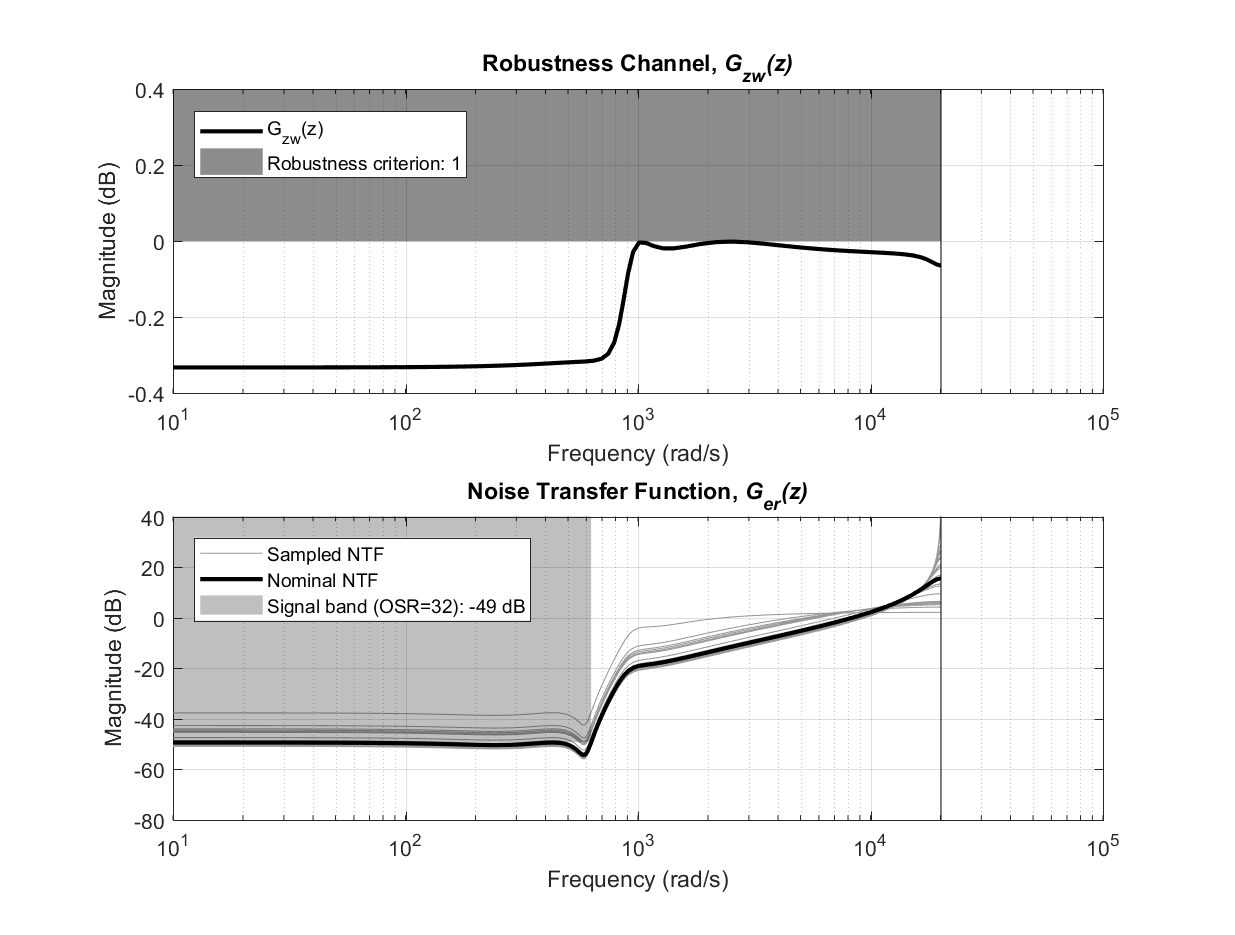
\includegraphics[height=6cm]{ntf-robust}
	\caption{The noise transfer function generated with the root locus stability criterion and associated optimization targets.}
\end{figure}

\end{frame}

\begin{frame}{Root Locus Stability Criterion iii}

\begin{figure}
	\centering
	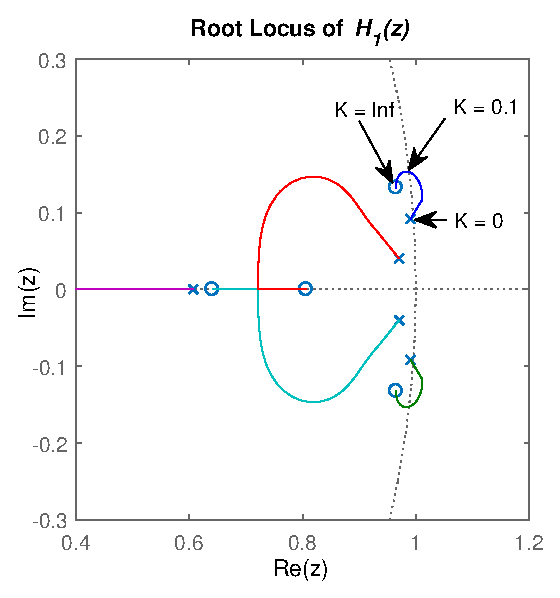
\includegraphics[height=6cm]{rl-robust}
	\caption{The root locus for the design produced when $\left[k_l, k_h\right] = \left[0.1, \infty\right)$.}
\end{figure}

\end{frame}
}

{\setbeamercolor{background canvas}{bg=white}

\begin{frame}{$\mathcal{H}_2$ Stability Criterion i}
\begin{figure}
	\begin{NoHyper}
		\begin{center}
			\begin{tikzpicture}
				\pgfplotsset{set layers}
				\begin{axis}[
					width=1.8in,
					title={\textbf{Trade-off with $\mathcal{H}_2$ Stability Criterion}},
					scale only axis,
					xmin=1,xmax=2.8,
					ymin=60,ymax=100,
					axis y line*=left,
					xlabel={$||G_{er}(z)||_2^2$},
					ylabel={Maximum SQNR (dB) \ref{plt:msqnr3}},
					]
					\addplot[solid,mark=*,mark options={fill=white}] table [x=h22,y=maxSqnr,col sep=comma] {data/comparison-h2-2.csv};
					\label{plt:msqnr3}
					\addplot[mark=*,mark options={fill=black}] coordinates {(1.7872483786618, 79.9)};
				\end{axis}
				\begin{axis}[
					width=1.8in,
					scale only axis,
					xmin=1,xmax=2.8,
					ymin=-14,ymax=0,
					axis y line*=right,
					axis x line=none,
					ylabel style={align=center},
					ylabel={Simulated MSIA, relative to FS (dB) \ref{plt:msia3-1}\\ Predicted MSIA, relative to FS (dB) \ref{plt:msia3-2}},
					]
					\addplot[solid,draw=gray,mark=square*,mark options={fill=white}] table [x=h22,y=msia,col sep=comma] {data/comparison-h2-2.csv};
					\label{plt:msia3-1}
					\addplot[solid,draw=gray,mark=triangle*,mark options={fill=white,scale=1.5}] table [x=h22,y=targetdBopt,col sep=comma] {data/comparison-h2-2.csv};
					\label{plt:msia3-2}
					\addplot[mark=square*,draw=gray,mark options={fill=gray}] coordinates {(1.7872483786618, -2.1)};
					\addplot[mark=triangle*,draw=gray,mark options={fill=gray}] coordinates {(1.7872483786618, -3.22498532140599)};
				\end{axis}
			\end{tikzpicture}
		\end{center}
	\end{NoHyper}
	\caption{The performance (maximum simulated SQNR) and stability achieved with the modulator design for $\mathcal{H}_2$ norm goals.}
\end{figure}

\end{frame}

%\begin{frame}{$\mathcal{H}_2$ Stability Criterion II}
%
%\begin{figure}
%	\centering
%	\includegraphics[height=6cm]{ntf-h2}
%	\caption{The noise transfer function generated with the $\mathcal{H}_2$ stability criterion and associated optimization targets.}
%\end{figure}
%
%\end{frame}

\begin{frame}{$\mathcal{H}_2$ Stability Criterion ii}

\begin{figure}
	\centering
	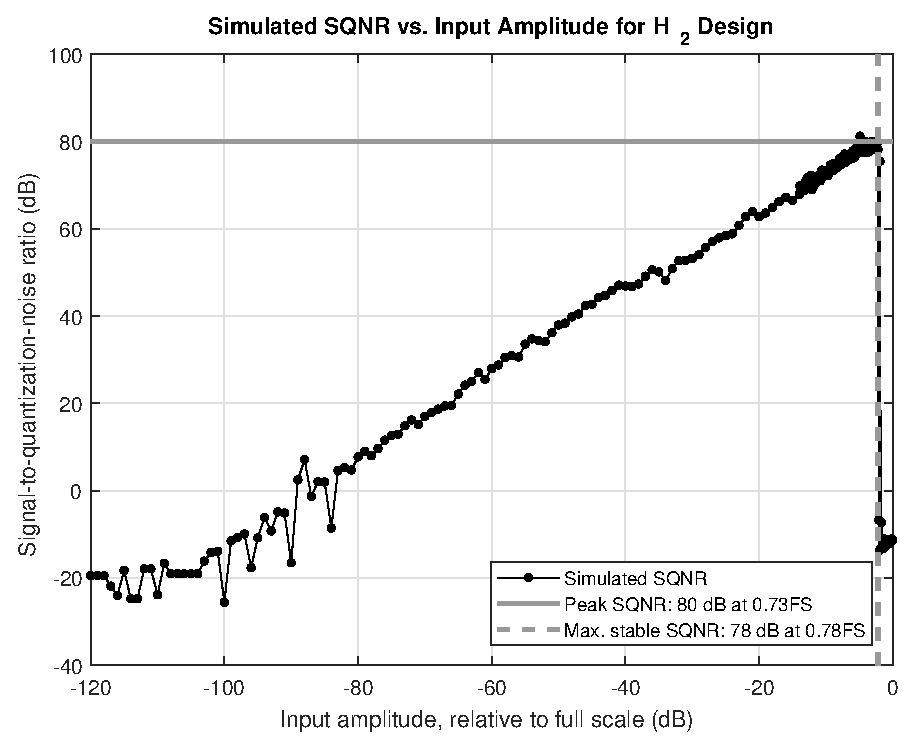
\includegraphics[height=6cm]{sqnr-h2}
	\caption{Simulation data for the modulator generated with the $\mathcal{H}_2$ stability criterion.}
\end{figure}

\end{frame}
}

{\setbeamercolor{background canvas}{bg=white}
\begin{frame}{$\ell_1$ Stability Criterion i}

\begin{figure}
	\begin{NoHyper}
		\begin{center}
			\begin{tikzpicture}
				\pgfplotsset{set layers}
				\begin{axis}[
					width=1.8in,
					title={\textbf{Trade-off with $\ell_1$ Stability Criterion}},
					scale only axis,
					xmin=2,xmax=6,
					ymin=40,ymax=80,
					axis y line*=left,
					xlabel={$||G_{er}(z)||_\star$},
					ylabel={Maximum SQNR (dB) \ref{plt:msqnr4}},
					]
					\addplot[solid,mark=*,mark options={fill=white}] table [x=star,y=maxSqnr,col sep=comma] {data/comparison-l1.csv};
					\label{plt:msqnr4}
					\addplot[mark=*,mark options={fill=black}] coordinates {(4, 58.87)};
				\end{axis}
				\begin{axis}[
					width=1.8in,
					scale only axis,
					xmin=2,xmax=6,
					ymin=-16,ymax=0,
					axis y line*=right,
					axis x line=none,
					ylabel style={align=center},
					ylabel={Simulated MSIA, relative to FS (dB) \ref{plt:msia4-1}\\ Guaranteed MSIA from $\star$-norm (dB) \ref{plt:msia4-2}\\ Guaranteed MSIA from $\ell_1$ norm (dB) \ref{plt:msia4-4}},
					]
					\addplot[solid,draw=gray,mark=square*,mark options={fill=white}] table [x=star,y=msia,col sep=comma] {data/comparison-l1.csv};
					\label{plt:msia4-1}
					\addplot[solid,draw=gray,mark=triangle*,mark options={fill=white,scale=1.5}] table [x=star,y=msiaExpStardB,col sep=comma] {data/comparison-l1.csv};
					\label{plt:msia4-2}
					\addplot[solid,draw=gray,mark=pentagon*,mark options={fill=white,scale=1.25}] table [x=star,y=msiaExpOptdB,col sep=comma] {data/comparison-l1.csv};
					\label{plt:msia4-4}
					\addplot[mark=square*,draw=gray,mark options={fill=gray}] coordinates {(4, 0)};
					\addplot[mark=pentagon*,draw=gray,mark options={fill=gray,scale=1.25}] coordinates {(4, -3.332007102)};
				\end{axis}
			\end{tikzpicture}
		\end{center}
	\end{NoHyper}
	\caption{The performance (maximum simulated SQNR) and stability achieved with the modulator design for $\star$-norm goals.}
\end{figure}

\end{frame}

\begin{frame}{$\ell_1$ Stability Criterion ii}

\begin{figure}
	\centering
	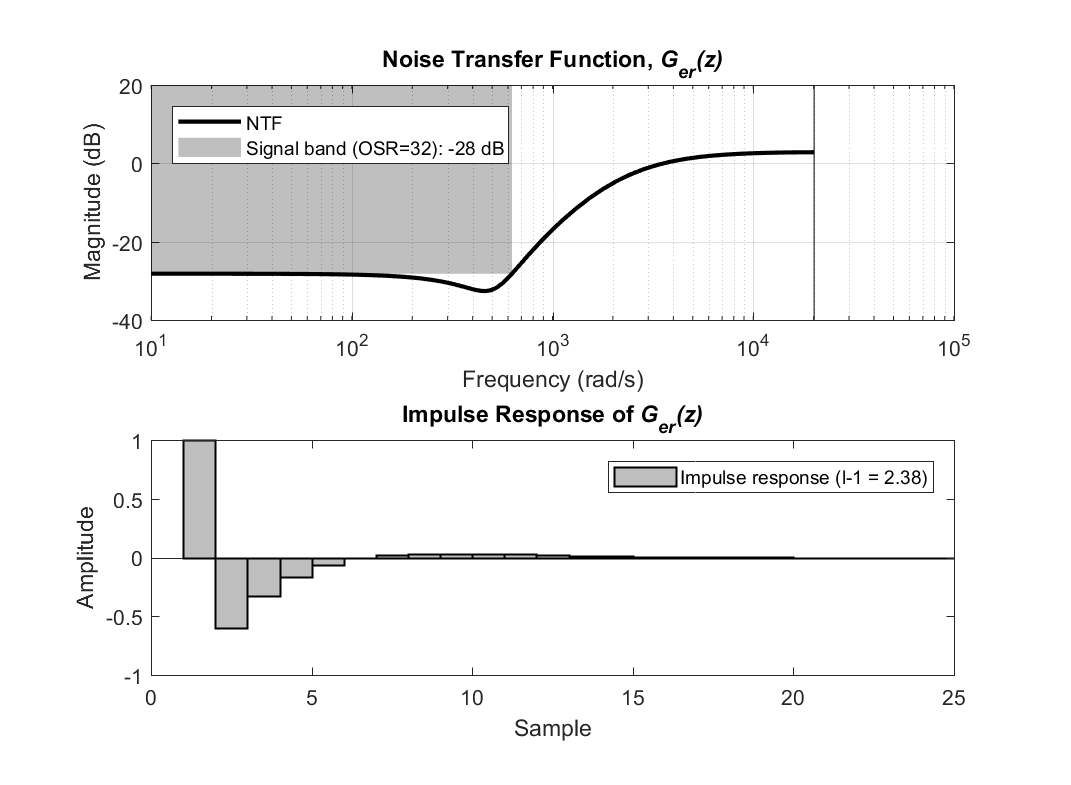
\includegraphics[height=6cm]{ntf-l1}
	\caption{The noise transfer function generated with the $\ell_1$ stability criterion and associated optimization targets.}
\end{figure}

\end{frame}

\begin{frame}{Summary of Examples}

\begin{table}
	\caption{The performance and stability observations from simulations done on modulators designed using each stability criterion.}
	\begin{tabular}{p{1.8cm} p{2.4cm} p{1.9cm} p{1.8cm} p{0.9cm}}
		\toprule
		\textbf{Type} & \textbf{Peak SQNR} & \textbf{MSIA (pred.)} & \textbf{MSIA (sim.)} & \textbf{LRIA} \\
		\midrule
		\texttt{DSToolbox} & \SI{87}{\deci\bel} & N/A & 0.76 FS & \SI{-96}{\deci\bel} \\
		$\mathcal{H}_\infty$ & \SI{86}{\deci\bel} at 0.62 FS & N/A & 0.71 FS & \SI{-91}{\deci\bel} \\
		Root locus & \SI{66}{\deci\bel} & N/A & 1 FS & \SI{-52}{\deci\bel} \\
		$\mathcal{H}_2$ & \SI{78}{\deci\bel} at 0.73 FS & 0.69 FS & 0.78 FS & \SI{-84}{\deci\bel} \\
		$\ell_1$ & \SI{59}{\deci\bel} & 0.68 FS & 1 FS & \SI{-41}{\deci\bel} \\
		\bottomrule
	\end{tabular}
\end{table}

\end{frame}
}

\section{Conclusion}

\begin{frame}{Contributions}

\begin{itemize}
	\item Development of an algorithm that unites sigma delta modulator design using $\mathcal{H}_\infty$, $\mathcal{H}_2$, and $\ell_1$ stability criteria with the GKYP performance goal supporting both FIR and IIR filters.
	\item Extending the LMI system from \cite{Li2014} to be compatible with other channels of the augmented system.
	\item Modelling the quantizer gain as an uncertainty and using optimization to enforce stability for a range of quantizer gains.
	\item Presenting a proof-of-concept of using this work to directly design continuous-time loop filters.
\end{itemize}

\end{frame}

{\setbeamercolor{palette primary}{fg=black, bg=yellow}
\begin{frame}[standout]
  Questions?
\end{frame}
}

%\appendix
%
%\begin{frame}[fragile]{Backup slides}
%  Sometimes, it is useful to add slides at the end of your presentation to
%  refer to during audience questions.
%I
%  The best way to do this is to include the \verb|appendixnumberbeamer|
%  package in your preamble and call \verb|\appendix| before your backup slides.
%
%  \themename will automatically turn off slide numbering and progress bars for
%  slides in the appendix.
%\end{frame}

\begin{frame}[allowframebreaks]{References}

	\bibliographystyle{ieeetr}
	\bibliography{/Users/brett/Documents/Mendeley_Desktop/BibTeX/library}

\end{frame}

\end{document}

